
\section{Hardware Design Component}

An ambulance is equipped with multitudes of technology, ranging from oxygen tanks to IVs \cite{AmericanCollegeofSurgeonsCommitteeonTrauma}. In our discussions with paramedics, we have found there is currently no tool available to track and record a patients real-time vitals. According to paramedics, such a tool would be of useful.

To adequately track the vitals of a patient, there are 2 main hardware components required; the transmitter and the sensor.

\subsection{Sensor}
As this is a preliminary design, only one vital will be tracked as proof of modality, so the focus will be on heart rate.
A simple heart rate sensor will be constructed consisting of an infrared and red wavelength emitter and receiver as well as an amplification circuit.
The 2 LEDS are pulsed on the skin of the patient and the reflectance of both wavelengths is measured by detectors. IR and red light scatter differently
depending on the amount of blood in the skin at that time and the detectors pick up the reflected light from both and output the corresponding current and
voltage. This is then amplified and is sent to a microcontroller.

To decrease the size of the overall sensor, an ATmega microcontroller can be used with the appropriate capacitors, oscillators, and power source to avoid the
use of a full Arduino board. This chip will receive signals in from the pulse circuit and can calculate the heart rate, creating a pulse wave to show heart activity. These signals can then be sent out through a Wi-Fi Transceiver module to the user’s mobile device.
 \subsection{Transmitter}
 All modern communication devices, such as tablets and mobile phones, can connect to auxiliary devices via Bluetooth and Wi-Fi. Bluetooth communication has
 limitations on how many devices can be connected to a parent device at any given time with the ideal number being 4. \cite{apple1} As the primary use for this device
  will be for mass accidents, being limited to 4 patients per device is impractical. Wireless internet networks such as Wi-Fi are less limited and allow for
  10 devices to be connected at a time when using a mobile hotspot source. When a paramedic is out in the field, a mobile internet source will be provided
  from a mobile hotspot and will have the ability to have 10 devices actively communicating with it at a time. This also allows for information to be sent to
  the hospital in real time whereas Bluetooth communication would be limited to when the patient has already reached the hospital. Because of this we have
  chosen to connect to our sensors through Wi-Fi with the receiver being the devices own internal Wi-Fi receiver.
 To transmit the data from the pulse oximetry sensor to the mobile device, a serial Wi-Fi transceiver module will be used. With both devices connected to
 the same wireless network, data will able to be sent serially from the sensor to the host device.
 \begin{figure}[h]
  \centering
  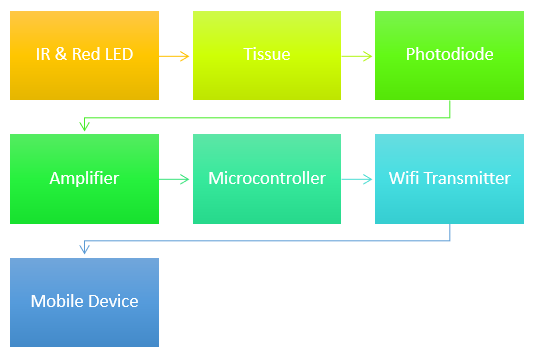
\includegraphics[width=\linewidth]{hardwareFlowchart.PNG}
  \captionsetup{format=hang}
  \caption[Hardware Block Diagram]{Block Diagram of Hardware Components}
  \label{fig:HwardwareDiagram}
\end{figure}
